% Options for packages loaded elsewhere
% Options for packages loaded elsewhere
\PassOptionsToPackage{unicode}{hyperref}
\PassOptionsToPackage{hyphens}{url}
\PassOptionsToPackage{dvipsnames,svgnames,x11names}{xcolor}
%
\documentclass[
  letterpaper,
  DIV=11,
  numbers=noendperiod]{scrreprt}
\usepackage{xcolor}
\usepackage{amsmath,amssymb}
\setcounter{secnumdepth}{5}
\usepackage{iftex}
\ifPDFTeX
  \usepackage[T1]{fontenc}
  \usepackage[utf8]{inputenc}
  \usepackage{textcomp} % provide euro and other symbols
\else % if luatex or xetex
  \usepackage{unicode-math} % this also loads fontspec
  \defaultfontfeatures{Scale=MatchLowercase}
  \defaultfontfeatures[\rmfamily]{Ligatures=TeX,Scale=1}
\fi
\usepackage{lmodern}
\ifPDFTeX\else
  % xetex/luatex font selection
\fi
% Use upquote if available, for straight quotes in verbatim environments
\IfFileExists{upquote.sty}{\usepackage{upquote}}{}
\IfFileExists{microtype.sty}{% use microtype if available
  \usepackage[]{microtype}
  \UseMicrotypeSet[protrusion]{basicmath} % disable protrusion for tt fonts
}{}
\makeatletter
\@ifundefined{KOMAClassName}{% if non-KOMA class
  \IfFileExists{parskip.sty}{%
    \usepackage{parskip}
  }{% else
    \setlength{\parindent}{0pt}
    \setlength{\parskip}{6pt plus 2pt minus 1pt}}
}{% if KOMA class
  \KOMAoptions{parskip=half}}
\makeatother
% Make \paragraph and \subparagraph free-standing
\makeatletter
\ifx\paragraph\undefined\else
  \let\oldparagraph\paragraph
  \renewcommand{\paragraph}{
    \@ifstar
      \xxxParagraphStar
      \xxxParagraphNoStar
  }
  \newcommand{\xxxParagraphStar}[1]{\oldparagraph*{#1}\mbox{}}
  \newcommand{\xxxParagraphNoStar}[1]{\oldparagraph{#1}\mbox{}}
\fi
\ifx\subparagraph\undefined\else
  \let\oldsubparagraph\subparagraph
  \renewcommand{\subparagraph}{
    \@ifstar
      \xxxSubParagraphStar
      \xxxSubParagraphNoStar
  }
  \newcommand{\xxxSubParagraphStar}[1]{\oldsubparagraph*{#1}\mbox{}}
  \newcommand{\xxxSubParagraphNoStar}[1]{\oldsubparagraph{#1}\mbox{}}
\fi
\makeatother


\usepackage{longtable,booktabs,array}
\usepackage{calc} % for calculating minipage widths
% Correct order of tables after \paragraph or \subparagraph
\usepackage{etoolbox}
\makeatletter
\patchcmd\longtable{\par}{\if@noskipsec\mbox{}\fi\par}{}{}
\makeatother
% Allow footnotes in longtable head/foot
\IfFileExists{footnotehyper.sty}{\usepackage{footnotehyper}}{\usepackage{footnote}}
\makesavenoteenv{longtable}
\usepackage{graphicx}
\makeatletter
\newsavebox\pandoc@box
\newcommand*\pandocbounded[1]{% scales image to fit in text height/width
  \sbox\pandoc@box{#1}%
  \Gscale@div\@tempa{\textheight}{\dimexpr\ht\pandoc@box+\dp\pandoc@box\relax}%
  \Gscale@div\@tempb{\linewidth}{\wd\pandoc@box}%
  \ifdim\@tempb\p@<\@tempa\p@\let\@tempa\@tempb\fi% select the smaller of both
  \ifdim\@tempa\p@<\p@\scalebox{\@tempa}{\usebox\pandoc@box}%
  \else\usebox{\pandoc@box}%
  \fi%
}
% Set default figure placement to htbp
\def\fps@figure{htbp}
\makeatother





\setlength{\emergencystretch}{3em} % prevent overfull lines

\providecommand{\tightlist}{%
  \setlength{\itemsep}{0pt}\setlength{\parskip}{0pt}}



 


\KOMAoption{captions}{tableheading}
\makeatletter
\@ifpackageloaded{bookmark}{}{\usepackage{bookmark}}
\makeatother
\makeatletter
\@ifpackageloaded{caption}{}{\usepackage{caption}}
\AtBeginDocument{%
\ifdefined\contentsname
  \renewcommand*\contentsname{Table of contents}
\else
  \newcommand\contentsname{Table of contents}
\fi
\ifdefined\listfigurename
  \renewcommand*\listfigurename{List of Figures}
\else
  \newcommand\listfigurename{List of Figures}
\fi
\ifdefined\listtablename
  \renewcommand*\listtablename{List of Tables}
\else
  \newcommand\listtablename{List of Tables}
\fi
\ifdefined\figurename
  \renewcommand*\figurename{Figure}
\else
  \newcommand\figurename{Figure}
\fi
\ifdefined\tablename
  \renewcommand*\tablename{Table}
\else
  \newcommand\tablename{Table}
\fi
}
\@ifpackageloaded{float}{}{\usepackage{float}}
\floatstyle{ruled}
\@ifundefined{c@chapter}{\newfloat{codelisting}{h}{lop}}{\newfloat{codelisting}{h}{lop}[chapter]}
\floatname{codelisting}{Listing}
\newcommand*\listoflistings{\listof{codelisting}{List of Listings}}
\makeatother
\makeatletter
\makeatother
\makeatletter
\@ifpackageloaded{caption}{}{\usepackage{caption}}
\@ifpackageloaded{subcaption}{}{\usepackage{subcaption}}
\makeatother
\usepackage{bookmark}
\IfFileExists{xurl.sty}{\usepackage{xurl}}{} % add URL line breaks if available
\urlstyle{same}
\hypersetup{
  pdftitle={Satria Wisnu Wibowo},
  pdfauthor={18222087 Satria Wisnu Wibowo},
  colorlinks=true,
  linkcolor={blue},
  filecolor={Maroon},
  citecolor={Blue},
  urlcolor={Blue},
  pdfcreator={LaTeX via pandoc}}


\title{Satria Wisnu Wibowo}
\usepackage{etoolbox}
\makeatletter
\providecommand{\subtitle}[1]{% add subtitle to \maketitle
  \apptocmd{\@title}{\par {\large #1 \par}}{}{}
}
\makeatother
\subtitle{Portfolio Asesmen II-2100 KIPP}
\author{18222087 Satria Wisnu Wibowo}
\date{2025-10-19}
\begin{document}
\maketitle

\renewcommand*\contentsname{Table of contents}
{
\hypersetup{linkcolor=}
\setcounter{tocdepth}{2}
\tableofcontents
}

\bookmarksetup{startatroot}

\chapter*{Selamat Datang}\label{selamat-datang}
\addcontentsline{toc}{chapter}{Selamat Datang}

\markboth{Selamat Datang}{Selamat Datang}

\begin{figure}[H]

{\centering \pandocbounded{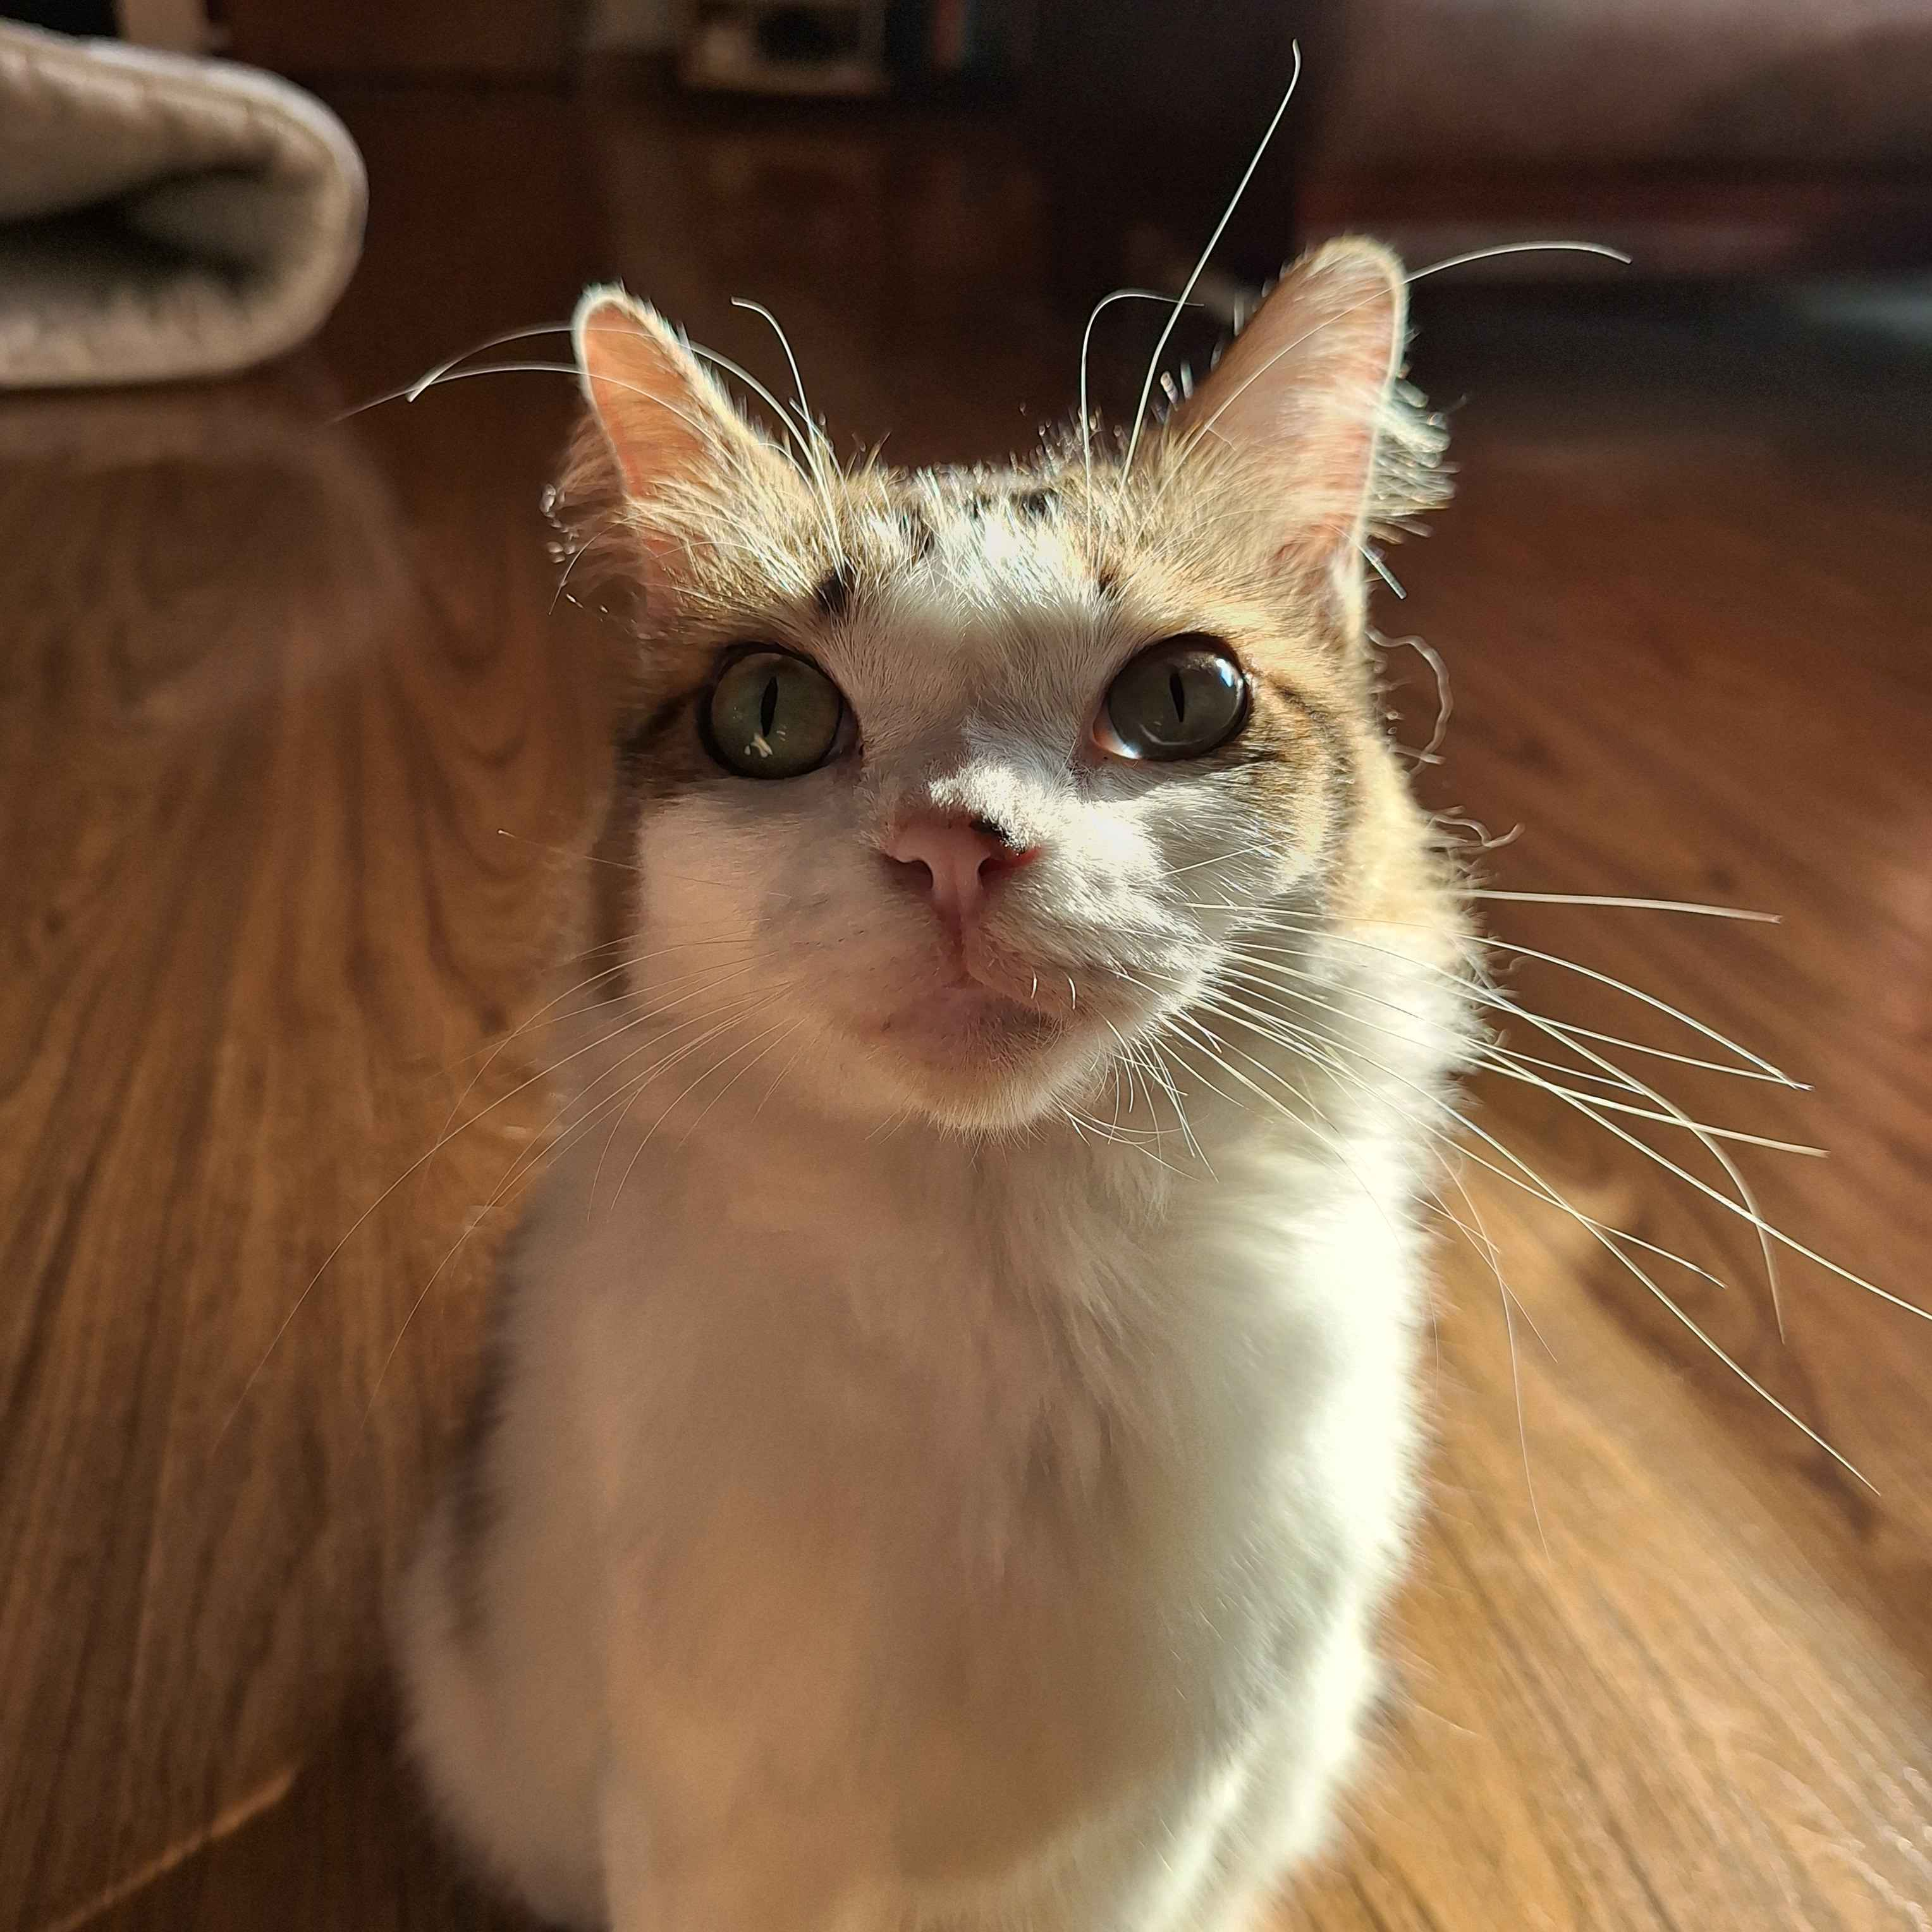
\includegraphics[keepaspectratio]{images/20240713_073218.jpg}}

}

\caption{About Me}

\end{figure}%

Halo! Saya Satria Wisnu Wibowo. Selamat datang di repositori tugas mata
kuliah II2100 - Komunikasi Interpersonal.

Di sini, saya mendokumentasikan perjalan saya dalam mempelajari dan
mengasah keterampilan Komunikasi interpersonal melalui teks, karya, dan
refleksi pribadi.

Catatan: Semua yang saya tulis di sini merupakan hasil pemikiran singkat
dan eksploratif, sehingga mungkin tidak sepenuhnya mencerminkan diri
saya sebenarnya.

\bookmarksetup{startatroot}

\chapter{UTS-1 All About Me}\label{uts-1-all-about-me}

\begin{figure}[H]

{\centering 
\includegraphics[width=0.5\linewidth,height=\textheight,keepaspectratio]{All_About_me/../images/HamiltonLogo.jpg}

}

\caption{Hamilton}

\end{figure}%

Saya Satria Wisnu Wibowo, biasa dipanggil Satria, merupakan mahasiswa
Sistem dan Teknologi Informasi yang selalu penasaran bagaimana ide bisa
diubah menjadi sesuatu yang nyata. Saya suka melihat sesuatu yang
abstrak, seperti bagaimana orang berpikir atau mengapa suatu ide kecil
bisa menjadi hal besar dan mencoba menuangkannya melalui coding, membuat
visual interaktif, menggambar, atau sekedar menulis cerita pendek yang
sering tidak selesai.

Dalam berkomunikasi, saya lebih suka mendengarkan daripada didengarkan.
Bukan karena saya pendiam (mungkin karena itu juga), tetapi karena saya
percaya bahwa setiap orang memiliki alasan di balik cara mereka
berkomunikasi, dan memahami itu membantu saya menjalin hubungan lebih
baik.

Lucunya, saya sering dibilang ``terlalu serius'', padahal sebenarnya
saya hanya butuh waktu lebih lama untuk merasa nyaman. Ketika sudah
nyaman, saya bisa menjadi pembicara yang mungkin berbicara lebih banyak
dari yang diharapkan.

Ada satu kutipan dari \emph{Hamilton: The Musical} yang cukup melekat di
kepala saya yaitu ``I am not throwing away my shot!''

Kalimat itu bukan hanya tentang ambisi besar, tetapi tentang keberanian
untuk mencoba bicara, bahkan ketika suara kita belum terlalu lantang.
Saya sering merasa seperti itu, tidak ingin melewatkan kesempatan untuk
belajar, berinteraksi, atau sekadar menunjukkan bahwa saya ada, meskipun
pelan.

Bagi saya, mengenal diri sendiri adalah perjalanan panjang. Saya ingin
terus belajar memahami diri dan orang lain, agar bisa berkomunikasi
dengan lebih jujur, bermakna, dan mungkin lebih berani mengambil
``shot'' saya sendiri.

\bookmarksetup{startatroot}

\chapter{UTS-2 My Songs for You}\label{uts-2-my-songs-for-you}

\section{Just Learn to Live}\label{just-learn-to-live}

``Just Learn to Live'' ini merupakan sebuah karya yang merefleksikan
cara saya menjalani hidup. Lagu ini menceritakan tentang
\textbf{bagaimana seharusnya menjalani hidup}, bukanlah hanya sekedar
``mencari tempat'' yang sesuai, tetapi juga dengan mempelajari bagaimana
``tempat'' yang kita tempati sekarang dapat menjadi sesuai bagi kita.
Baik dengan menyesuaikan diri kita atau membuatnya sesuai bagi kita.

Catatan: Untuk mempercepat proses pembuatan, \textbf{pembuatan lagu
menggunakan Udio AI} berdasarkan lirik yang ditulis berdasarkan narasi
tentang pribadi saya.

Your browser does not support the audio element.

\subsection{Lirik}\label{lirik}

\begin{quote}
\textbf{{[}Verse 1{]}}\\
I used to wait for someone to call my name,\\
Standing quiet at the edge of the game.\\
Every thought too loud inside my head,\\
Every word rehearsed but left unsaid.

\textbf{{[}Pre-Chorus{]}}\\
Then I walked into a place with no plans,\\
No charts, no rules, just helping hands.\\
And somehow that chaos taught me more,\\
Than all the walls I built before.

\textbf{{[}Chorus{]}}\\
I don't need to die anywhere else,\\
Just learn to live inside myself.\\
Not chasing noise, or flashing fame,\\
Just leaving light when they say my name.

\textbf{{[}Verse 2{]}}\\
Fast to learn, slow to belong,\\
Guess I've been humming the same old song.\\
Thinking too much, feeling too deep,\\
Dreaming of something that I could keep.

\textbf{{[}Pre-Chorus{]}}\\
I used to think legacy meant gold,\\
But now I see --- it's stories told.\\
In every code, in every hand,\\
In every life I help to stand.

\textbf{{[}Chorus{]}}\\
I don't need to die anywhere else,\\
Just build a world that holds itself.\\
Not chasing crowns or saving grace,\\
Just meaning carved in time and space.

\textbf{{[}Bridge{]}}\\
Maybe I'm not loud, but I am clear,\\
Every quiet step still brought me here.\\
And if I fade when the lights are gone,\\
My echoes will hum this same old song.

\textbf{{[}Final Chorus{]}}\\
I don't need to die anywhere else,\\
Just learn to live inside myself.\\
Not chasing stars that burn away,\\
Just building something that will stay.
\end{quote}

\bookmarksetup{startatroot}

\chapter{UTS-3 My Stories for You}\label{uts-3-my-stories-for-you}

\section{Cerita dari Panggung yang Tak Pernah
Diam}\label{cerita-dari-panggung-yang-tak-pernah-diam}

\begin{figure}[H]

{\centering 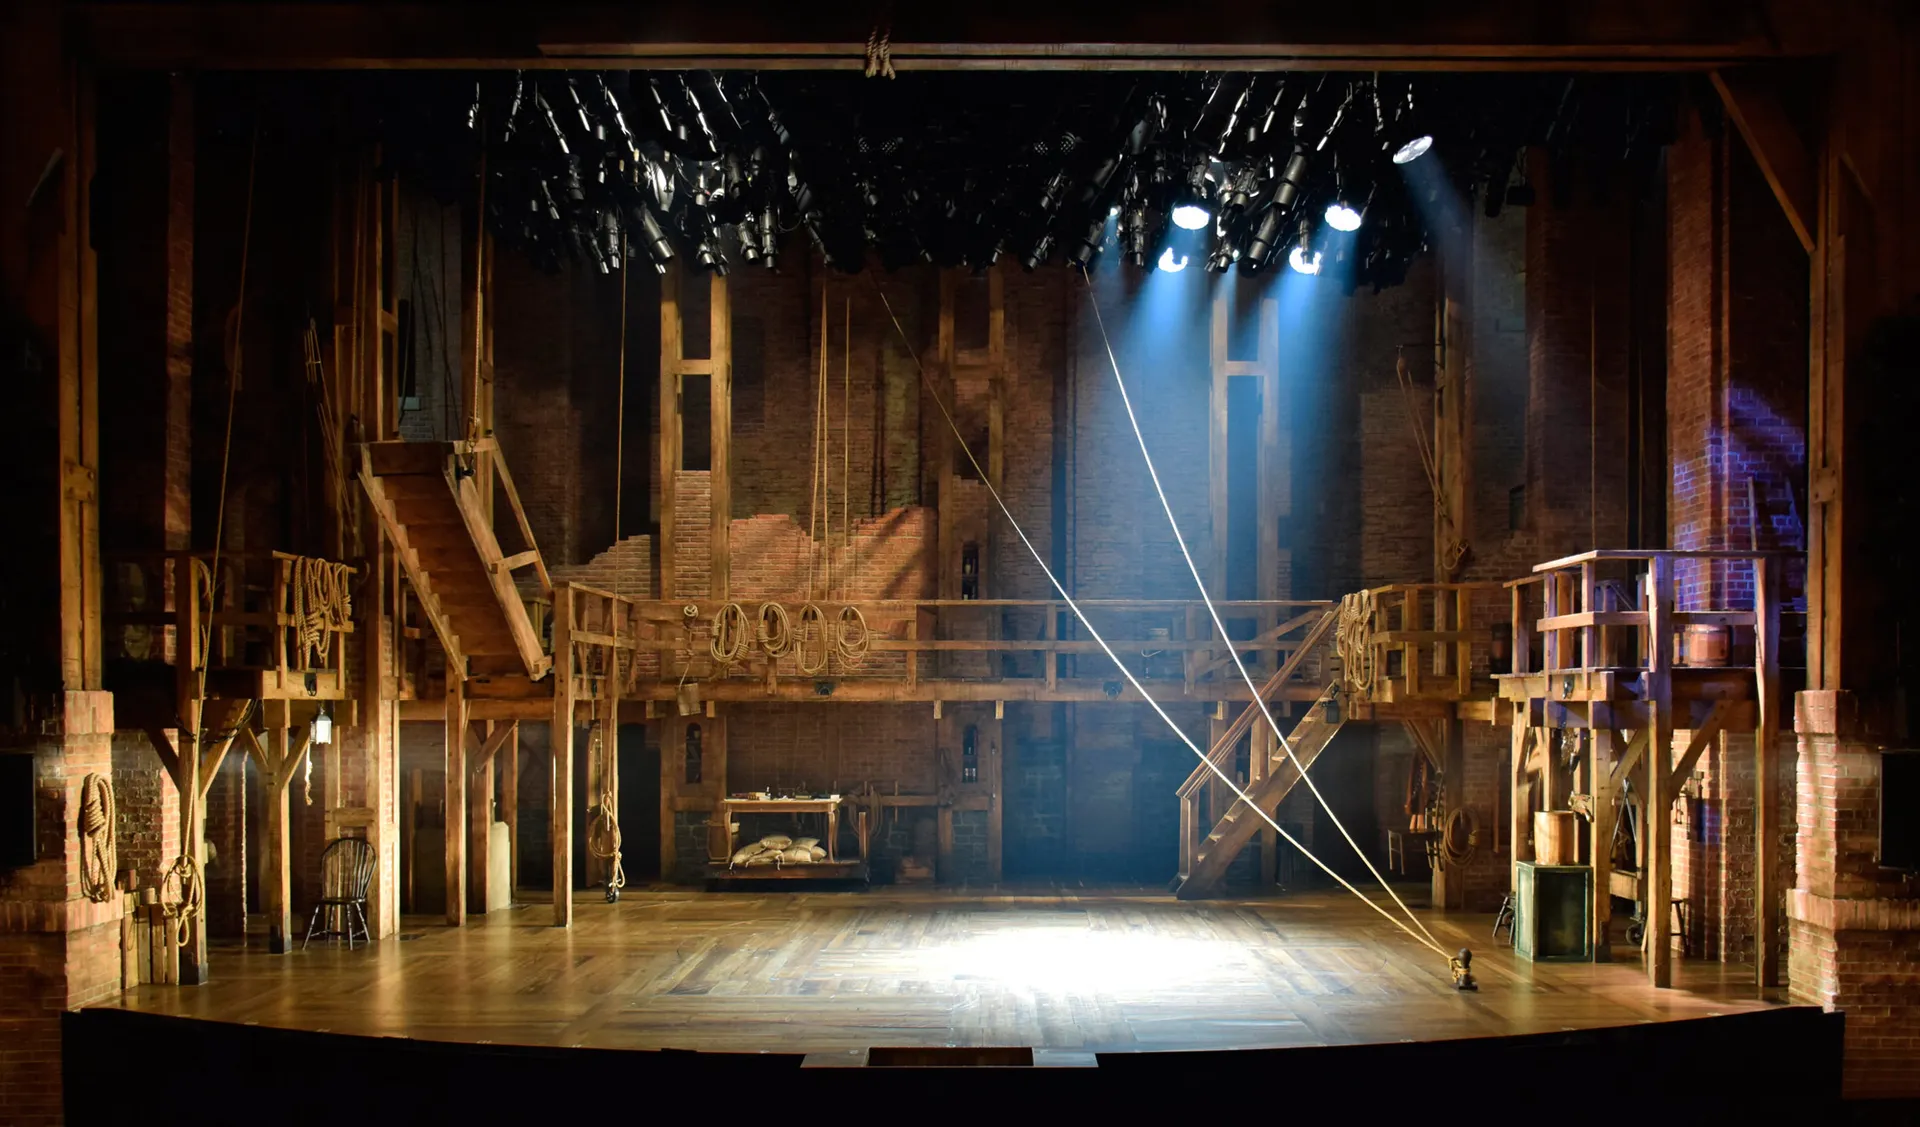
\includegraphics[width=0.95\linewidth,height=\textheight,keepaspectratio]{My_Stories_for_You/../images/hamiltonSet.jpg}

}

\caption{Courtesy of David Korins Design}

\end{figure}%

Untuk kamu yang mungkin sedang takut mencoba.

Saya ingin bercerita tentang Hamilton: The Musical. Bukan sekedar
musikal tentang sejarah Amerika, tetapi tentang \textbf{bagaimana
seseorang berani bercerita dengan caranya sendiri}, bahkan ketika orang
lain menganggap idenya terlalu aneh, terlalu baru, terlalu berani.

Lin-Manuel Miranda, penulis musikal ini, mendapat ide untuk menulis
musikal ini saat dia sedang membaca biografi Alexander Hamilton karya
Ron Chernow. Ia bukan orang pertama yang membaca buku itu, tetapi
mungkin orang satu-satunya yang melihatnya sebagai hip-hop opera tentang
perjuangan hidup, ambisi, dan identitas.

Saya terobsesi pada bagaimana ia \textbf{menghidupkan sejarah dengan
bahasa masa kini}, dan bagaimana setiap liriknya terasa seperti napas,
jujur, cepat, berirama, tetapi juga rapuh.

Di balik panggung Broadway, ada ratusan jam latihan, revisi naskah,
bahkan kegagalan. Namun justru di sanalah letak keajaiban muncul, di
antara rasa takut, lelah, dan keyakinan bahwa cerita ini layak untuk
diceritakan.

Mungkin itulah mengapa saya selalu terinspirasi oleh Hamilton. Bukan
hanya karena kontennya saja, tetapi karena pesan yang merealisasikan
konten itu, bahwa keberanian bukan tentang berdiri di tengah sorotan,
melainkan tentang menulis satu bait pertama meski belum tahu bagaimana
akhir lagunya nanti.

\section{Ketika Dunia Kerja Tidak Seperti di
Buku}\label{ketika-dunia-kerja-tidak-seperti-di-buku}

\begin{figure}[H]

{\centering 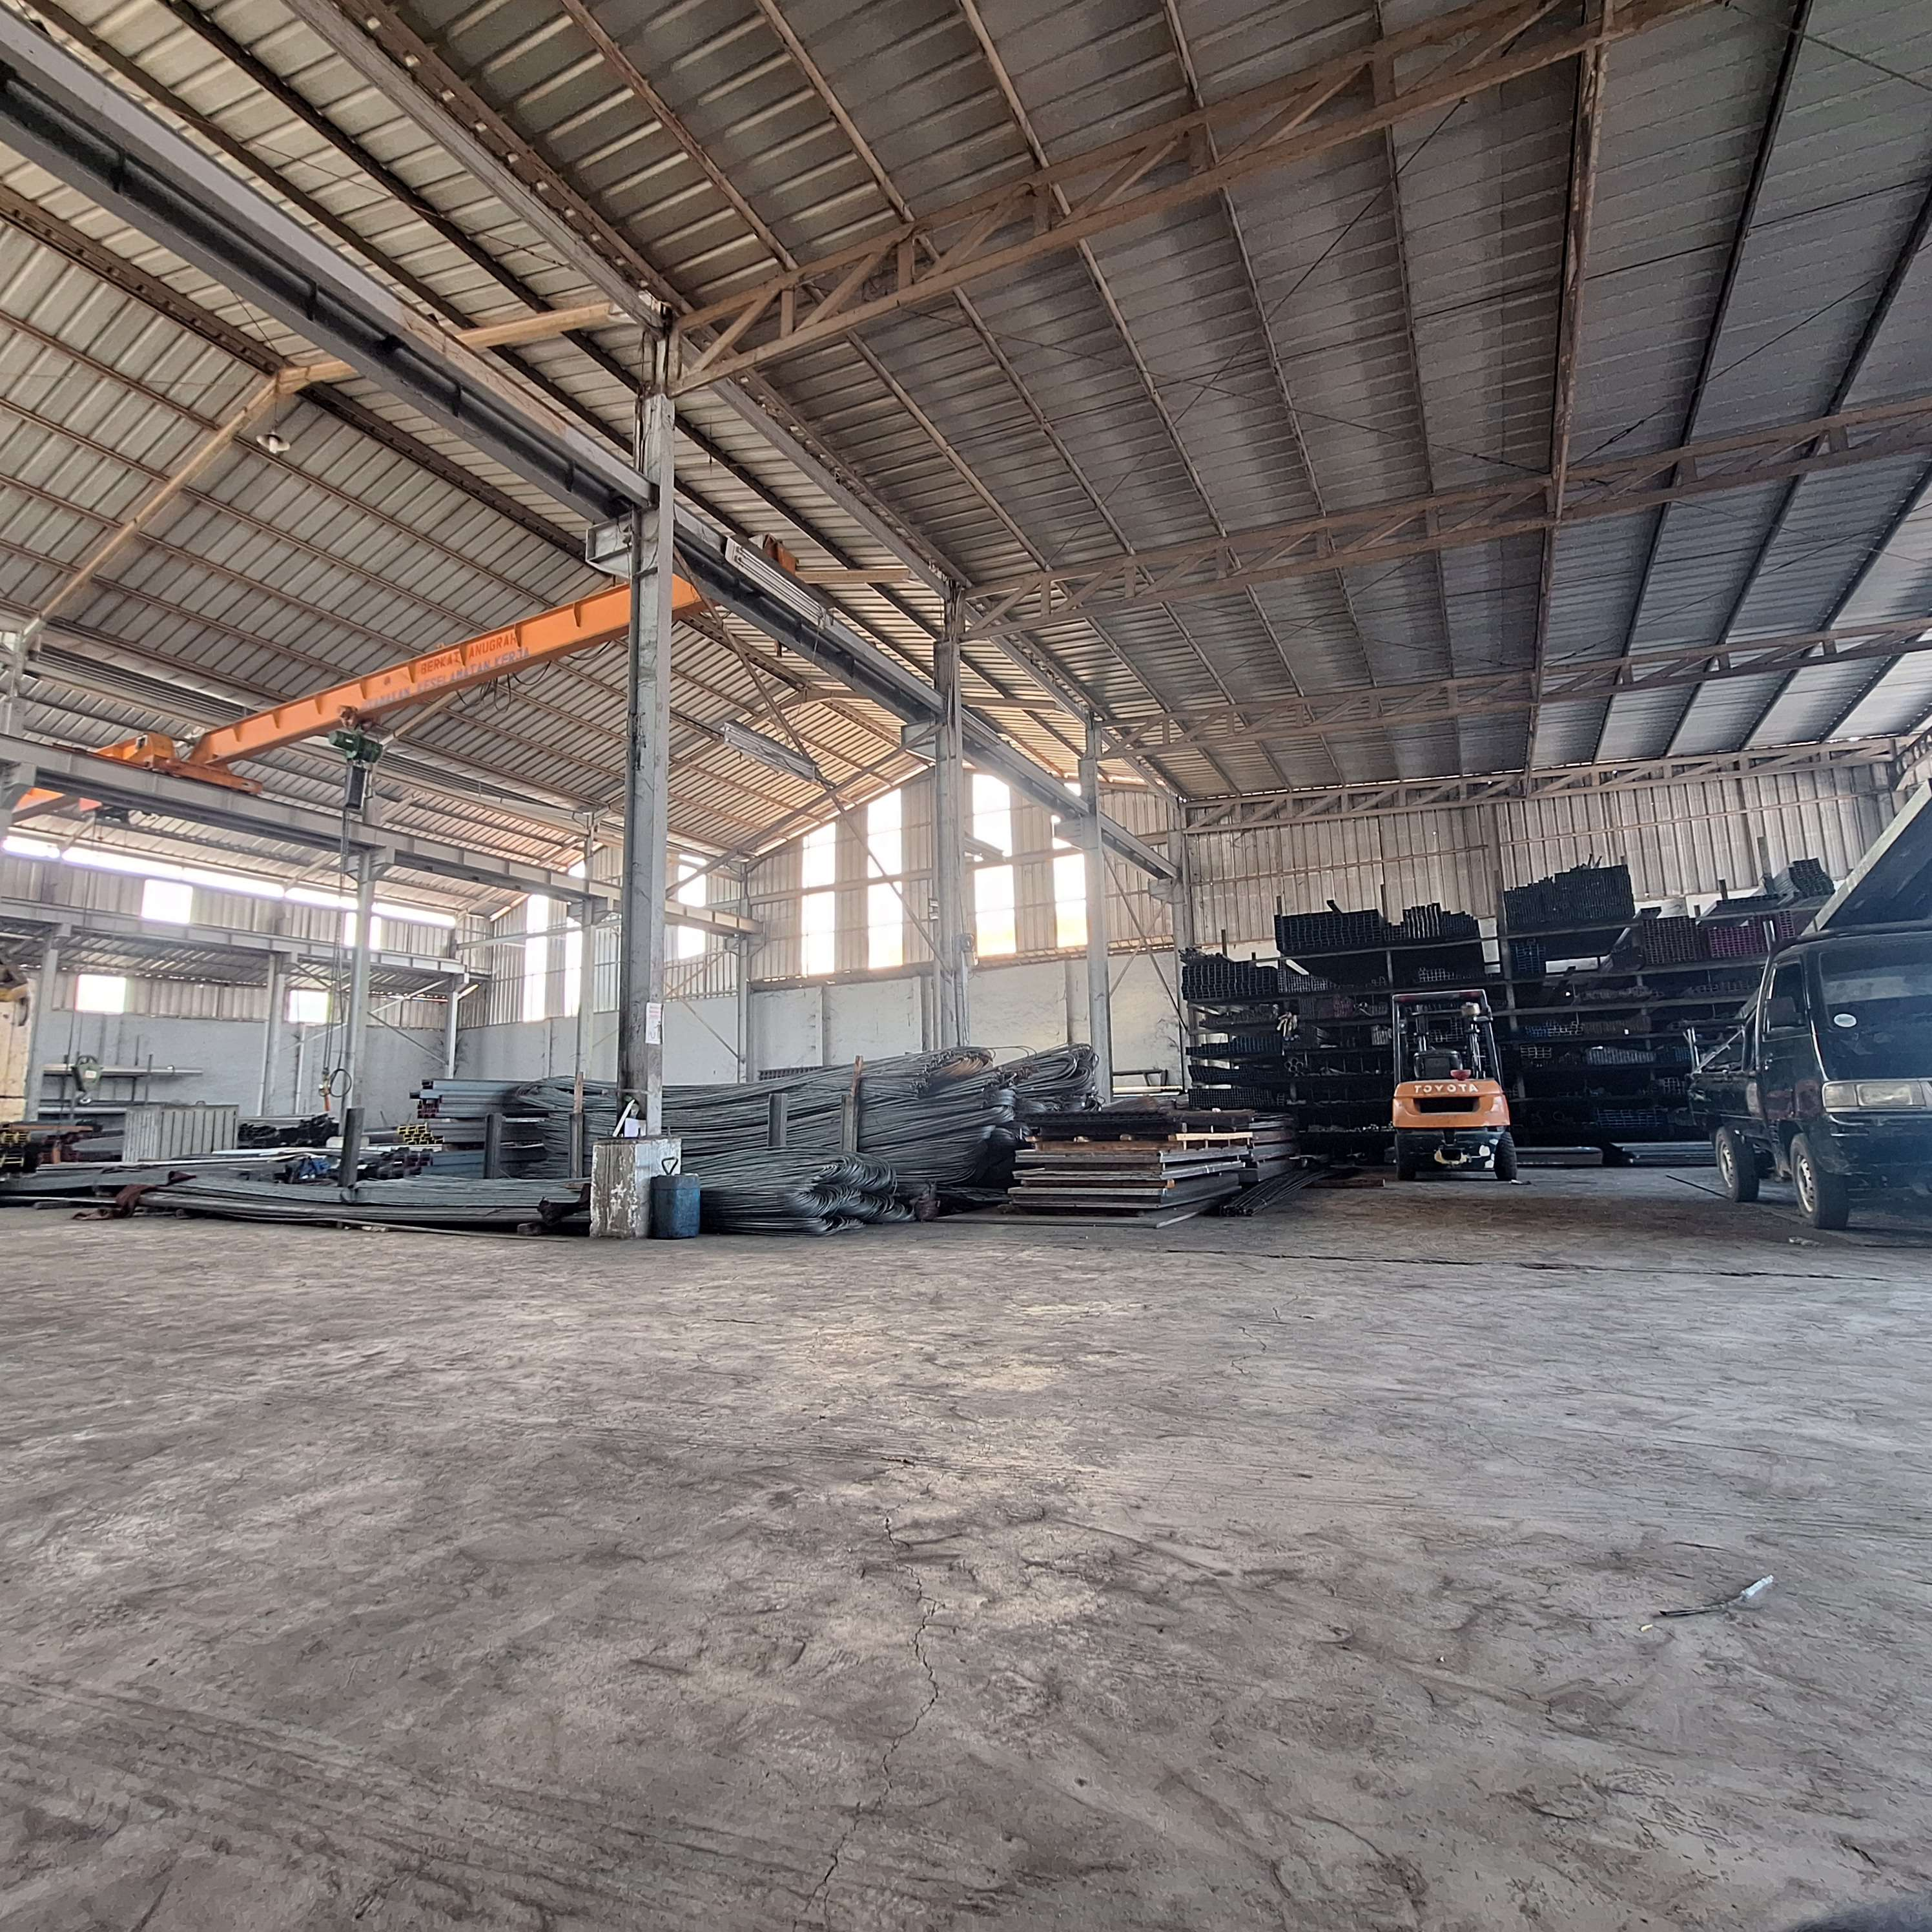
\includegraphics[width=0.5\linewidth,height=\textheight,keepaspectratio]{My_Stories_for_You/../images/gudang.jpg}

}

\caption{August 16, 2025}

\end{figure}%

Saya masih ingat hari pertama kerja praktik. Rasanya seperti dilempar ke
kolam yang dingin tanpa pelampung. Saya tidak mengenal siapapun di
tempat itu, dan untuk seseorang yang sejak kecil lebih nyaman diam di
sudut ruangan sampai ada tangan yang menjangkau, itu menegangkan.

Sejujurnya, saya datang dengan ekspektasi yang sangat korporat. Saya
membayangkan jadwal meeting mingguan dan laporan harian. Saya sudah
menyiapkan catatan dan mempersiapkan diri semantap mungkin untuk segala
pertanyaan, persis seperti karyawan magang ideal di kantor besar.

Mungkin saya hanya takut secara berlebihan, tetapi begitu saya tiba dan
beberapa hari berjalan, saya sadar bahwa ekspektasi terhadap lingkungan
korporat itu tidak terlalu kental. Tempat kerja praktik merupakan sebuah
toko dengan ritme hidup yang jauh lebih cair dan spontan.

Awalnya saya kebingungan. Tidak ada laporan harian yang perlu diisi,
tidak ada arahan terkait target minggu ini, dan tidak ada email atau
pesan yang perlu dibalas dengan ``baik, noted''. Semua orang bekerja
dengan caranya masing-masing, berbeda dengan teori budaya kerja yang
dijelaskan pada perkuliahan.

Namun, justru di sana lah saya belajar sesuatu yang tidak pernah saya
temukan di dunia korporat, kehangatan komunikasi manusia yang tidak
tertulis. Bagaimana memahami rekan kerja tanpa instruksi formal,
bagaimana membantu tanpa diminta, bagaimana menyesuaikan diri dengan
ritme orang lain.

Perlahan saya belajar membuka diri. Saya belajar bercanda, belajar tanpa
takut terdengar bodoh, belajar menyesuaikan diri dengan gaya komunikasi
yang lebih langsung dan spontan. Sesekali memang canggung, saya pernah
menunggu ``briefing'' padahal rekan lain sudah sibuk sejak pagi, tetapi
lama-lama saya ikut terbawa.

Sekarang saya menyadari bahwa tempat yang sederhana itu justru memberi
saya pelajaran yang paling berharga. Bahwa komunikasi tidak hanya soal
profesionalitas, tetapi juga empati. Bahwa bekerja bukan sekedar
mengikuti struktur dan standar, tetapi juga beradaptasi dengan manusia
di dalamnya.

Kerja praktik saya mungkin tidak terlihat ``formal'', tetapi di sana lah
saya benar-benar belajar menjadi pribadi yang lebih terbuka dan mandiri.

\bookmarksetup{startatroot}

\chapter{UTS-4 My SHAPE (Spiritual Gifts, Heart, Abilities, Personality,
Experiences)}\label{uts-4-my-shape-spiritual-gifts-heart-abilities-personality-experiences}

\section{Piagam Diri}\label{piagam-diri}

\begin{longtable}[]{@{}
  >{\raggedright\arraybackslash}p{(\linewidth - 2\tabcolsep) * \real{0.4783}}
  >{\raggedright\arraybackslash}p{(\linewidth - 2\tabcolsep) * \real{0.5217}}@{}}
\toprule\noalign{}
\begin{minipage}[b]{\linewidth}\raggedright
Kategori
\end{minipage} & \begin{minipage}[b]{\linewidth}\raggedright
Deskripsi
\end{minipage} \\
\midrule\noalign{}
\endhead
\bottomrule\noalign{}
\endlastfoot
\textbf{Signature Strengths (Kekuatan Khas)} & Dapat memahami sesuatu
dengan cepat begitu saya ``menangkap polanya''. \\
\textbf{Heart (Nilai Inti \& Motivasi Intrinsik)} & Saya memiliki
motivasi untuk menciptakan sesuatu yang bermakna dan berguna bagi orang
lain. \\
\textbf{Aptitudes \& Acquired Skills (Bakat \& Keterampilan)} & 1. Mampu
membuat desain yang efektif dan estetik bahkan di luar domain keahlian
saya.2. Memiliki rasa ingin tahu tinggi dan belajar dengan
cepat.Memiliki empati dan kepekaan terhadap dinamika tim. \\
\textbf{Personality (Kepribadian)} & Saya merupakan seorang INTJ, dengan
kecenderungan berpikir strategis dan mandiri. Saya suka merencanakan
sesuatu dengan matang. Namun, saya juga belajar untuk lebih terbuka
terhadap spontanitas dan kolaborasi, karena saya sadar bahwa ide besar
tidak tumbuh sendiri. \\
\textbf{Experiences (Pengalaman Hidup)} & Saya menyadari bahwa peran
orang tua dalam mengambil keputusan terkait kehidupan saya bukanlah
sekedar paksaan semata, bagi mereka, mungkin itu adalah keputusan
terbaik bagi saya, bagi saya, mungkin juga tidak, tetapi hasil ke
depannya tetap menjadi tanggung jawab saya untuk menghasilkan yang
terbaik dari keputusan tersebut. \\
\end{longtable}

\section{Pernyataan Misi Pribadi}\label{pernyataan-misi-pribadi}

\begin{quote}
Saya ingin menjadi seseorang yang meninggalkan suatu ``legacy'', sebuah
warisan atau nilai yang tetap hidup bahkan setelah saya tiada.
\end{quote}

\section{Identitas Naratif}\label{identitas-naratif}

Saat ini, saya adalah seorang mahasiswa Sistem dan Teknologi Informasi
yang sangat tertarik pada hubungan antara teknologi, sosial, dan makna
di balik suatu karya. Saya senang menggabungkan logika dengan estetika,
terutama ketika hasilnya memberi manfaat bagi orang lain (H).

Sejak dulu, saya memiliki rasa ingin tahu yang tinggi untuk belajar
banyak hal di luar bidang yang saya tekuni. Hal ini memungkinkan saya
memahami sesuatu dengan cepat bahkan pada topik yang tidak saya kuasai
sebelumnya (S)(A). Walaupun ``trade-off''nya adalah saya tidak terlalu
mendalami apa-apa saja yang saya pahami, tetapi itu masih bisa diatasi
ke depannya.

Sebagai refleksi pribadi, saya juga belajar banyak dari pengalaman dalam
keluarga saya, di mana keputusan yang diambil orang tua mungkin tidak
selalu sejalan dengan keinginan saya, tetapi saya belajar untuk
bertanggung jawab terhadap hasilnya dan mencari makna di baliknya. Dari
situ saya memahami bahwa setiap keputusan hidup, baik yang saya pilih
sendiri maupun yang tidak, tetap bisa saya ubah menjadi kesempatan untuk
tumbuh (E).

Ke depan, saya ingin membangun ``legacy'', sesuatu yang tetap hidup
bahkan setelah saya tiada. Entah itu berupa karya, sistem, atau nilai
yang membantu orang lain berkembang. Jika bercerita tentang hubungan
semua ini ke perusahaan, saya ingin mengeksplorasi peluang di industri
pertambangan, khususnya di negara-negara dengan praktik pertambangan
modern seperti Australia. Saya percaya bahwa kombinasi antara kemampuan
strategis saya sebagai seorang INTJ, rasa ingin tahu yang tak pernah
padam, serta keinginan untuk menciptakan hal bermakna dapat membawa saya
menuju ke sana (P).

\bookmarksetup{startatroot}

\chapter{UTS-5 My Personal Reviews}\label{uts-5-my-personal-reviews}

Berikut cara saya melakukan review: menggunakan ChatGPT Saya mengattach
\href{skor_uts.pdf}{file promt ChatGPT}, disertai perintah : ``self
assess uts-1 sanpai uts-5 dari URL
`https://ii-2100.github.io/all-about-me/'\,''

ChatGPT melakukan self-assessment UTS-1 s.d. UTS-5 langsung dari laman
yang Anda berikan dan menilai memakai rubrik tugas UTS (skala 1--5 per
kriteria). Rekap skor siap diunduh sebagai CSV:
\href{sandbox:/mnt/data/UTS_self_assessment.csv}{Download CSV
ringkasan}.

\bookmarksetup{startatroot}

\chapter{Hasil Self-Assessment UTS (URL:
https://peabnj.github.io/all-about-me/)}\label{hasil-self-assessment-uts-url-httpspeabnj.github.ioall-about-me}

\section{Identifikasi}\label{identifikasi}

\begin{itemize}
\tightlist
\item
  Nama \& NIM penulis: \textbf{Satria Wisnu Wibowo -- 18222087} (tertera
  di halaman depan portofolio). ({[}II 2100{]}{[}1{]})
\item
  Penilai: \textbf{Self-assessment (Satria Wisnu Wibowo)}
\item
  Catatan cakupan:
\end{itemize}

\section{Tinjauan Umum}\label{tinjauan-umum}

Portofolio ini terdiri dari empat tugas utama (UTS-1 s.d. UTS-4) yang
masing-masing menunjukkan aspek berbeda dari komunikasi interpersonal
dan refleksi diri. Secara keseluruhan, karya ini mencerminkan upaya saya
untuk memahami diri sendiri, mengomunikasikannya secara artistik, dan
menghubungkannya dengan orang lain. Tiap tugas memiliki gaya dan
kekuatan tersendiri: UTS-1 berfokus pada narasi personal, UTS-2 pada
ekspresi emosional melalui lirik lagu, UTS-3 pada kisah reflektif, dan
UTS-4 pada pemetaan kekuatan dan nilai pribadi. Dari keseluruhan karya,
konsistensi orisinalitas dan kesadaran diri menjadi kekuatan utama,
sementara aspek teknis dan kedalaman inspirasi masih dapat ditingkatkan.

\begin{center}\rule{0.5\linewidth}{0.5pt}\end{center}

\section{Tinjauan Spesifik + Skor
(1--5)}\label{tinjauan-spesifik-skor-15}

\subsection{UTS-1 --- All About Me (di
beranda)}\label{uts-1-all-about-me-di-beranda}

\textbf{Skor per kriteria:} Orisinalitas \textbf{5}, Keterlibatan
\textbf{4}, Humor \textbf{3}, Wawasan/Insight \textbf{4} → \textbf{Total
16/20 (80\%)}.\\
\textbf{Alasan singkat:} Narasi ditulis dengan jujur dan bernuansa
introspektif. Saya mencoba menyeimbangkan antara kejujuran personal dan
gaya penceritaan yang ringan. Secara orisinal, tulisan ini kuat karena
menggambarkan cara berpikir saya sendiri.\\
\textbf{Saran perbaikan:} Humor bisa lebih eksploratif agar pembaca
lebih terlibat.

\subsection{UTS-2 --- My Songs for You}\label{uts-2-my-songs-for-you-1}

\textbf{Skor per kriteria:} Orisinalitas \textbf{4}, Keterlibatan
\textbf{4}, Humor \textbf{3}, Inspirasi \textbf{4} → \textbf{Total 15/20
(75\%)}.\\
\textbf{Alasan singkat:} Struktur lirik mengikuti pola verse dan
pre-chorus yang cukup rapi, dengan ritme emosional yang meningkat secara
bertahap. Nilai orisinalitas cukup tinggi karena lagu ini muncul dari
pengalaman pribadi.\\
\textbf{Saran perbaikan:} Inspirasi terasa, namun beberapa bagian masih
terdengar umum dan dapat diperdalam.

\subsection{UTS-3 --- My Stories for
You}\label{uts-3-my-stories-for-you-1}

\textbf{Skor per kriteria:} Orisinalitas \textbf{4}, Keterlibatan
\textbf{4}, Pengembangan Narasi \textbf{3}, Inspirasi \textbf{4} →
\textbf{Total 15/20 (75\%)}.\\
\textbf{Alasan singkat:} Dari sisi keterlibatan, cukup berhasil menjaga
perhatian pembaca. Inspirasi tersampaikan meski belum sangat mendalam.\\
\textbf{Saran perbaikan:} Memperkaya narasi dengan simbolisme dan sudut
pandang yang lebih kompleks.

\subsection{UTS-4 --- My SHAPE}\label{uts-4-my-shape}

\textbf{Skor per kriteria:} Orisinalitas \textbf{5}, Keterlibatan
\textbf{4}, Pengembangan Narasi \textbf{4}, Inspirasi \textbf{4} →
\textbf{Total 17/20 (85\%)}.\\
\textbf{Alasan singkat:} Visualisasi dengan tabel SHAPE membantu menata
refleksi dengan sistematis. Orisinalitas tinggi karena kontennya
bersumber langsung dari pengalaman pribadi.\\
\textbf{Saran perbaikan (prioritas):} Namun, aspek inspiratif bisa
diperkuat dengan mengaitkan temuan diri dengan tujuan jangka panjang.

\subsection{UTS-5 --- My Personal
Reviews}\label{uts-5-my-personal-reviews-1}

\textbf{Skor per kriteria:} Pemahaman Konsep , Analisis Kritis ,
Argumentasi (Logos) , Etos \& Empati , Rekomendasi → \textbf{Total /25
(\%)}.\\
\textbf{Alasan singkat:}\\
\textbf{Saran perbaikan:}

\begin{center}\rule{0.5\linewidth}{0.5pt}\end{center}

\section{Rekap Skor (ringkas)}\label{rekap-skor-ringkas}

\begin{itemize}
\tightlist
\item
  \textbf{UTS-1:} 16/20 → \textbf{80\%}
\item
  \textbf{UTS-2:} 15/20 → \textbf{75\%}
\item
  \textbf{UTS-3:} 15/20 → \textbf{75\%}
\item
  \textbf{UTS-4:} 17/20 → \textbf{85\%}
\item
  \textbf{UTS-5:} /25 → \textbf{\%}
\end{itemize}

\section{Saran Perbaikan Umum}\label{saran-perbaikan-umum}

Secara umum, keempat tugas menunjukkan konsistensi dalam gaya personal
dan ekspresi autentik. Saya telah mampu menampilkan kepribadian, nilai,
serta pemahaman interpersonal dengan cara yang jujur dan terarah. Namun,
untuk peningkatan ke depan, saya akan lebih memperhatikan unsur
dramatika, kedalaman pesan, dan eksplorasi media (visual/audio) agar
komunikasi lebih berkesan

\bookmarksetup{startatroot}

\chapter{UAS-1 My Concepts}\label{uas-1-my-concepts}

\bookmarksetup{startatroot}

\chapter{UAS-2 My Opinions}\label{uas-2-my-opinions}

\bookmarksetup{startatroot}

\chapter{UAS-3 My Innovations}\label{uas-3-my-innovations}

\bookmarksetup{startatroot}

\chapter{UAS-4 My Knowledge}\label{uas-4-my-knowledge}

\bookmarksetup{startatroot}

\chapter{UAS-5 My Professional
Reviews}\label{uas-5-my-professional-reviews}

\bookmarksetup{startatroot}

\chapter{Summary}\label{summary}

\bookmarksetup{startatroot}

\chapter*{References}\label{references}
\addcontentsline{toc}{chapter}{References}

\markboth{References}{References}

\phantomsection\label{refs}




\end{document}
